%% grundlagen.tex $Id: grundlagen.tex 28 2007-01-18 16:31:32Z bless $
%%

\chapter{Grundlagen}
\label{ch:Grundlagen}
%% ==============================

Dieses Kapitel führt Grundlagen ein, die für das Verständnis der
Arbeit notwendig sind. Dies sind zum einen die Kryptographie mit
öffentlichen Schlüsseln und das sich daraus ergebende Problem der
Authentifizierung öffentlicher Schlüssel. Ausserdem wird auf die
Funktionsweise der PGP-Software eingegangen.

Da der Fokus dieser Arbeit auf der Netzwerkstruktur des Web of Trust
liegt, werden die kryptographischen Grundlagen (Abschnitt
\ref{ch:Grundlagen:sec:PublicKeyCrypto}) und die Funktionsweise
der PGP-Software (Abschnitt \ref{ch:Grundlagen:sec:PGP}) nur in dem Ausmaß besprochen, das für die weitere
Arbeit nötig ist. Für detailliertere Darstellungen wird auf
entsprechende Literatur verwiesen.

Abschnitt \ref{sec:graph-und-netzw} definiert dann den
grundlegenden Begriff des Graphen und einige verwandte Begriffe und
führt dann die Methoden aus dem Bereich der Netzwerkanalyse ein, mit
denen die Struktur des Web of Trust untersucht wird.

Zu beachten ist, dass im Kapitel \ref{ch:Grundlagen} der Begriff
``Schlüssel'' einen kryptographischen Schlüssel im Allgemeinen
bezeichnet, während ab Kapitel \ref{ch:Methoden} damit
ausschließlich der öffentliche Teil eines OpenPGP-Schlüsselpaares
gemeint ist.

%% ==============================
\section{Kryptographie mit öffentlichen Schlüsseln}
%% ==============================
\label{ch:Grundlagen:sec:PublicKeyCrypto}

Dieser Abschnitt erläutert zunächst die Prinzipien symmetrischer
und asymmetrischer Kryptographie, geht dann auf das Problem der
Schlüsselverteilung bei asymmetrischer Verschlüsselung ein und
führt zu dessen Lösung die Konzepte Public Key Infrastructure
(PKI), X.509 und Web of Trust (WoT) ein. Die Darstellung beruht auf
\cite{Menezes1996}.

\subsection{Ziele von Kryptographie}
\label{sec:ziele-von-krypt}

Wir betrachten den Fall einer Nachricht, die über einen Kanal
transportiert wird. Im Kontext von Computernetzwerken, insbesondere
des Internets, muss im Allgemeinen davon ausgegangen werden, dass
unberechtigte Dritte in der Lage sind, Nachrichten auf einem Kanal
abzuhören, zurückzuhalten und zu verändern. \pagebreak[1] Menezes et
al. \cite{Menezes1996} definieren essentielle Ziele von
Informationssicherheit, die in diesem Fall relevant sind:\
\begin{description}
\item[Vertraulichkeit] Es soll sichergestellt werden, dass der Inhalt
  einer Nachricht nur berechtigten Kommunikationspartnern zugänglich
  ist.
\item[Authentizität] Eine Nachricht ist dann authentisch, wenn sie
  zweifelsfrei ihrem Absender zugeordnet werden
  kann. Authentifizierung betrifft also die Verifizierung des
  Ursprungs oder des Urhebers einer Nachricht. Dieses Problem betrifft
  nicht nur die Nachricht selbst, sondern auch Schlüsselmaterial.
\item[Integrität] Es soll sichergestellt werden, dass eine Nachricht
  während des Transports nicht verändert wurde, bzw. dass eine
  Veränderung nicht unbemerkt möglich ist.
\end{description}

\subsection{Prinzip}
\label{ch:Grundlagen:sec:PublicKeyCrypto:subsec:Prinzip}

\emph{Symmetrische Kryptographie} basiert auf einem \emph{Geheimnis}
oder \emph{Schlüssel}, der sowohl dem Absender als auch dem
Empfänger bekannt ist. Der gleiche Schlüssel wird dazu benutzt,
eine Nachricht zu verschlüsseln und sie zu entschlüsseln. Diese
Vorgänge können von jedem durchgeführt werden, der im Besitz des
Schlüssels ist.  Die Teilnehmer müssen also sicherstellen, dass
keine unberechtigten Dritten in den Besitz des Schlüssels gelangen
können. Ein Schlüssel kann natürlich bei einem direkten Treffen
ausgetauscht werden. Die Verteilung oder Vereinbarung eines
Schlüssels zwischen den Kommunikationspartnern ist aber dann
schwierig, wenn ein direkter Austausch beispielsweise aufgrund von
geographischer Entfernung nicht möglich ist und zwischen den
Kommunikationspartnern noch kein sicherer Kanal\footnote{Ein sicherer
  Kanal bezeichnet einen Kanal, auf dem die oben definierten
  Eigenschaften Vertraulichkeit, Authentizität und Integrität
  gewährleistet sind.} existiert. Dieses Problem wird als
\emph{Schlüsselverteilungsproblem} bezeichnet\cite{Menezes1996}.
Außerdem stellt sich das Problem, dass für jede Menge von
Kommunikationspartnern ein unterschiedlicher Schlüssel benötigt
wird. Wenn davon ausgegangen wird, dass nur jeweils zwei
Kommunikationspartner miteinander kommunizieren, wächst die Anzahl
der benötigten Schlüssel also quadratisch mit der Anzahl der
Teilnehmer.

Eine Methode, um das Problem der Schlüsselverteilung über einen
unsicheren Kanal zu lösen, bietet \emph{asymmetrische Kryptographie}
oder \emph{Public-Key-Kryptographie}. Dabei gibt es keinen einzelnen
Schlüssel, über den alle Kommunikationspartner
verfügen. Stattdessen verfügt jeder Teilnehmer über ein
\emph{Schlüsselpaar}, das aus einem \emph{privatem} und einem
\emph{öffentlichen} Schlüssel besteht. Zwischen diesen beiden
Schlüsseln muss ein mathematischer Zusammenhang bestehen. Der
private Schlüssel darf allerdings nicht mit akzeptablem Aufwand aus
dem öffentlichen Schlüssel ableitbar sein. Das entscheidende
Merkmal eines asymmetrischen Kryptographieschemas ist, dass der
Schlüssel, mit dem eine Nachricht verschlüsselt wird, nicht mit
dem Schlüssel identisch ist, mit dem sie wieder entschlüsselt
werden kann.

Asymmetrische Kryptographie kann benutzt werden, um die in Abschnitt
\ref{sec:ziele-von-krypt} definierten Ziele zu
gewährleisten. Vertraulichkeit wird erreicht, indem der Absender
einer Nachricht diese mit dem öffentlichen Schlüssel des
Empfängers verschlüsselt. Diese Nachricht kann dann nur mit dem
entsprechenden privaten Schlüssel des Empfängers entschlüsselt
werden. Um Authentizität und Integrität zu
gewährleisten, werden \emph{digitale Signaturen} verwendet, die von
einem Geheimnis (dem privaten Schlüssel) und der zu signierenden
Nachricht abhängen. Ein digitales Signaturschema besteht aus einer
Signaturverifizierungsfunktion und einer
Signaturerzeugungsfunktion. Gegeben ein asymmetrisches Schlüsselpaar
mit einem öffentlichen Schlüssel $k$ und einem privaten
Schlüssel $k^{-1}$ sowie eine Nachricht $m$ wird eine digitale
Signatur $d$ erzeugt, indem die Signaturerzeugungsfunktion auf
$k^{-1}$ und $m$ angewandt wird. Um die Signatur $d$ zur Nachricht $m$
zu überprüfen, wird die Verifizierungsfunktion auf $d$, $m$ und
den öffentlichen Schlüssel $k$ angewandt. Sie gibt an, ob es sich
um eine gültige Signatur bezüglich des zugehörigen privaten
Schlüssels $k^{-1}$ handelt oder nicht.

Der öffentliche Schlüssel kann öffentlich beliebig verfügbar
gemacht und über einen unsicheren Kanal transportiert werden. Der
private Schlüssel hingegen darf nur dem Besitzer bekannt sein, da
nur mit ihm die Operationen Entschlüsselung und Erstellung von
digitalen Signaturen möglich sind.

Asymmetrische Kryptographie löst das oben angesprochene
Skalierungsproblem, da nicht mehr ein Schlüssel für jedes Paar von
Kommunikationspartnern benötigt wird, sondern nur noch ein
Schlüsselpaar für jeden Teilnehmer.

\subsection{Authentisierung von Schlüsseln}
\label{ch:Grundlagen:sec:PublicKeyCrypto:subsec:KeyAuth}
Die Verteilung von öffentlichen Schlüsseln über unsichere
Kanäle scheint zwar zunächst das
Schlüsselverteilungsproblem zu lösen. Öffentliche Schlüssel
können über beliebige Wege verteilt werden, etwa per E-Mail, auf
Webseiten oder auf Keyservern (Abschnitt
\ref{sec:das-keys-netzw}). Allerdings tritt dann ein weiteres Problem
auf: Wie kann sichergestellt werden, dass ein öffentlicher
Schlüssel authentisch ist, er also tatsächlich von dem
vorgeblichen Besitzer stammt und dieser das Schlüsselmaterial
kontrolliert? 

Sei angenommen, dass Benutzer $B$ den öffentlichen Schlüssel von
Benutzer $A$ über einen unsicheren Kanal bezieht und dass keine
Vorkehrungen getroffen werden, um die Authentizität des Schlüssels
sicherzustellen. Ein aktiver Angreifer $M$ könnte dann den echten
Schlüssel von $A$ abfangen und durch einen Schlüssel ersetzen, der
zwar die Identität von $A$ trägt, aber unter der Kontrolle von $M$
steht. $M$ wäre dann in der Lage, Nachrichten zu entschlüsseln, die
von $B$ mittels des vermeintlich $A$ gehörenden Schlüssels
verschlüsselt wurden. $M$ könnte darüber hinaus solche Nachrichten mit
dem echten Schlüssel von $A$ verschlüsseln und sie weiter
schicken. Auf diese Weise bliebe der Angriff unbemerkt. Ein solcher
Angriff wird als \emph{Man-in-the-middle-Angriff} bezeichnet.

Natürlich kann die Authentizität eines Schlüssels überprüft
werden, wenn dieser bei einem persönlichen Treffen übergeben
wird. Im Kontext elektronischer Kommunikation ist dies jedoch im
Allgemeinen nicht möglich. Stattdessen m\"ussen sich die Beteiligten dafür auf einen
zuverlässigen Dritten (Trusted Third Party -- TTP) verlassen,
der die Authentizität der Schlüssels bestätigt. Eine TTP gibt
eine Zusicherung über die Bindung von einem öffentlichen
Schlüssel an eine Person oder allgemein eine Entität ab.

Diese Zusicherung hat die Form eines \emph{Zertifikats}. Ein
Zertifikat besteht aus einem Datenteil, der eine Identität (in Form
eines Namens), den zugehörigen öffentlichen Schlüssel sowie
eventuell zusätzliche Attribute enthält. Außerdem enthält ein
Zertifikat einen Signaturteil. Dieser besteht aus einer digitalen
Signatur über dem Datenteil, die mit dem Schlüssel der TTP
erstellt wurde. Die Authentizität eines Zertifikats kann also
überprüft werden, indem die Signatur auf dem Zertifikat mit dem
öffentlichen Schlüssel der TTP (welcher natürlich selbst
authentisch sein muss) überprüft wird.

Um sich auf die Zusicherungen der TTP verlassen zu können, muss ein
Benutzer dieser \emph{vertrauen}. Vertrauen bedeutet hier die Annahme,
dass die TTP stets korrekte Zusicherungen abgibt. Um eine korrekte
Zusicherung in Form eines Zertifikats für einen öffentlichen
Schlüssel abgeben zu können, muss die TTP überprüfen, dass der
Schlüssel tatsächlich der Person gehört, deren Identität auf
dem Schlüssel vermerkt ist. Außerdem muss sichergestellt werden,
dass diese Person auch im Besitz des entsprechenden privaten
Schlüssels ist.

Selbstverständlich kann die Authentizität des öffentlichen
Schlüssels einer TTP wiederum durch ein Zertifikat sichergestellt
werden. Außerdem kann ein öffentlicher Schlüssel Zertifikate
für mehrere andere Schlüssel abgeben und für einen
öffentlichen Schlüssel können mehrere Zertifikate
existieren. Auf diese Weise ergibt sich im Allgemeinen ein
\emph{gerichteter Graph} der als \emph{Zertifikatsgraph} bezeichnet
wird.

\subsubsection{Hierarchische Public-Key-Infrastruktur mit X.509}
\label{ch:Grundlagen:sec:PublicKeyCrypto:subsec:KeyAuth:subsubsec:PKI}

Infrastrukturen für die sichere Verteilung von öffentlichen
Schlüsseln (Public-Key-Infrastrukturen -- PKI) lassen sich
dahingehend unterscheiden, welche Instanzen für das Ausstellen von
Zertifikaten zuständig sind. Eine Möglichkeit besteht darin, diese
Funktion exklusiv zentralen, Instanzen, so genannten \emph{Certificate
  Authorities}, zuzuweisen. Diese stellen bei der Ausstellung eines
Zertifikates sicher, dass der tatsächliche Besitzer des Schlüssels
mit dem angegebenen Besitzer identisch ist. In einem solchen Modell
sind die Teilnehmer hierarchisch angeordnet. 

Ein Beispiel für ein solches Modell ist eine
Public-Key-Infrastruktur nach dem X.509-Standard. In einer solchen PKI
sind Certificate Authorities hierarchisch in einem Baum
angeordnet. Jede CA zertifiziert diejenigen CAs, die in diesem Baum
unterhalb von ihr liegen. Normale Benutzer stellen selbst keine Zertifikate
aus, ihre öffentlichen Schlüssel bilden in diesem Baum also die
Blätter.

Certificate Authorities muss natürlich vertraut werden. Allerdings
haben einzelne Benutzer im Kontext von X.509-PKIs üblicherweise
wenig Einfluss darauf, welche CAs als vertrauenswürdig betrachtet
werden. In einer Organisation kann eine Richtlinie bestimmen, welche
Certificate Authorities Zertifikate ausstellen dürfen. Diese CAs sind
dann implizit vertrauenswürdig. Die meisten Anwender müssen jenen
Certificate Authorities vertrauen, deren Wurzelzertifikate als Teil
des Webbrowsers oder des Betriebssystems ausgeliefert werden.

Im Kontext von X.509 werden Certificate Authorities meistens von
staatlichen Organisationen oder Unternehmen betrieben, deren
Geschäftsmodell aus der Ausstellung von Zertifikaten gegen
Gebühren besteht. 

\subsection{Kryptographische Hashfunktionen}
\label{sec:krypt-hashf}

Eine grundlegende kryptographische Primitive sind
\emph{kryptographische Hashfunktionen}. Kryptographische
Hashfunktionen sind unter anderem ein entscheidender Baustein für
digitale Signaturschemata.

Eine Hashfunktion $h$ ist eine Abbildung von Binärstrings beliebiger
Länge auf Binärstrings einer festen Länge $n$. Die Ausgabe
$h(x)$ eines Binärstrings $x$ wird als \emph{Hashwert} (oder als
\emph{Fingerabdruck}) von $x$ bezeichnet. Übliche Kriterien für
eine gute Hashfunktion sind eine annähernde Gleichverteilung der
Hashwerte und eine möglichst geringe Wahrscheinlichkeit von
Kollisionen. Eine Kollision tritt dann auf, wenn $h(x) = h(y)$ für
zwei Eingaben $x$ und $y$ gilt.

Für eine kryptographische Hashfunktion werden zusätzliche
Eigenschaften gefordert. Es darf nicht mit akzeptablem
Berechnungsaufwand möglich sein, zwei Binärstrings $x_1$ und $x_2$
zu berechnen, so dass $h(x_1) = h(x_2)$ gilt. Diese Eigenschaft wird
als \emph{Kollisionsresistenz} bezeichnet. Außerdem muss die Funktion
resistent gegen \emph{Urbild-Angriffen} sein, d.h. es darf mit
akzeptablem Aufwand nicht möglich sein, zu einem Hashwert $y$ einen
Binärstring $x$ zu berechnen, so dass $h(x) = y$ gilt.


\section{PGP/GnuPG}
\label{ch:Grundlagen:sec:PGP}

PGP ist ein Softwarepaket, das unterschiedliche kryptographische
Methoden mit einem Fokus auf asymmetrischer Kryptographie zur
Verschlüsselung von E-Mails implementiert.  Die ursprüngliche
Version von PGP wurde von Phil Zimmerman entwickelt. Der Quellcode von
PGP wurde von Anfang an der Allgemeinheit zur Verfügung
gestellt. PGP wird seit 1996 als kommerzielles Produkt vertrieben,
blieb aber trotzdem kostenlos verfügbar \cite{wiki:pgp}. Seit 1998
ist das verwendete Nachrichten- und Schlüsselformat durch den RFC
2440 \cite{Callas1998} und seit 2007 durch den überarbeiteten RFC
4880 \cite{Callas2007} standardisiert. Seit 1999 existiert mit
GnuPG \cite{Gnupg2010} eine freie Implementierung von OpenPGP unter der
GNU General Public Licence, deren Entwicklung zeitweise vom deutschen
Bundesministerium für Wirtschaft und Technologie gefördert
wurde. GnuPG scheint inzwischen die am meisten verbreitete
OpenPGP-Implementierung zu sein.

PGP benutzt asymmetrische Kryptographie für Verschlüsselung und
digitale Signaturen und bietet damit ein Werkzeug, um Vertraulichkeit,
Authentizität etc. von Nachrichten zu erreichen. Die häufigste
Anwendung von PGP ist die Verschlüsselung und Signierung von
E-Mail-Nachrichten. Es kann aber auch benutzt werden, um beliebige
Dokumente und Dateien zu verschlüsseln und zu signieren.

Wie die meisten kryptographischen Systeme, die asymmetrische Verfahren
benutzen, ist PGP/GnuPG ein hybrides System. Die asymmetrischen
Schlüssel werden nur benutzt, um einen symmetrischen
Sitzungsschlüssel zu verschlüsseln, mit dem wiederum der
eigentliche Nachrichteninhalt verschlüsselt wird. Der Grund dafür
liegt unter anderem darin, dass symmetrische Verfahren in der Regel
deutlich schneller sind als asymmetrische Verfahren.

PGP und GnuPG implementieren eine Vielzahl von symmetrischen und
asymmetrischen Verschl\"usselungsalgorithmen sowie
Hashalgorithmen. GnuPG erzeugte bis zum Jahr 2009 in der
Standardeinstellung DSA/ElGamal-Schlüssel. Seit 2009 werden
standardm\"assig Schl\"ussel nach dem RSA-Verfahren erzeugt (siehe Abschnitt
\ref{sec:result-key-properties}).

OpenPGP-Schlüssel können mit einem Ablaufdatum versehen
werden. Auch einzelne Teile eines Schlüssels, etwa einzelne UserIDs
oder Signaturen, können ein Ablaufdatum erhalten. Ein Schlüssel
kann aus verschiedenen Gründen nicht mehr benutzbar sein: Er kann
kompromittiert worden sein, das Schlüsselmaterial oder eine
Passphrase können verloren gegangen sein oder er kann schlichtweg
durch einen anderen Schlüssel ersetzt worden sein. In solchen
Fällen kann ein Schlüssel \emph{widerrufen} werden, indem eine
spezielle Widerrufssignatur durch den Besitzer auf dem Schlüssel
angebracht wird. Ein abgelaufener oder widerrufener Schlüssel kann
zwar noch benutzt werden, um Nachrichten zu entschlüsseln und
Signaturen zu verifizieren. Er ist aber nicht mehr für
Verschlüsselungs- und Signierungsoperationen verwendbar.

\subsection{Web of Trust}
\label{ch:Grundlagen:sec:PublicKeyCrypto:subsec:KeyAuth:subsubsec:WOT}

Für die Authentifizierung von öffentlichen Schlüsseln benutzt
PGP eine dezentrale Alternative zu dem in Abschnitt
\ref{ch:Grundlagen:sec:PublicKeyCrypto:subsec:KeyAuth:subsubsec:PKI}
beschriebenen hierarchischen und zentralen
Modell \cite{Ashley1999}. Die Fähigkeit, Zertifikate auszustellen,
ist dabei nicht auf Certificate Authorities beschränkt. Stattdessen
ist jeder Benutzer in der Lage, Zertifikate für öffentliche
Schlüssel auszustellen. Ein öffentlicher Schlüssel kann von
beliebig vielen Teilnehmern zertifiziert werden. Damit ergibt sich
für die Zertifikate nicht nur ein Baum, sondern tatsächlich ein
allgemeiner gerichteter Zertifikatsgraph. Dieser Graph wird als
\emph{Web of Trust}\footnote{Dieser Begriff ist irreführend, da der
  Zertifikatsgraph zunächst keine Informationen über Vertrauen
  enthält, sondern tatsächlich nur aus Zertifikaten besteht. Er
  wird in dieser Arbeit trotzdem benutzt, da er in der Literatur
  etabliert ist.} bezeichnet.

Da jeder Teilnehmer Zertifikate ausstellen kann, stellt jeder
Teilnehmer potentiell eine Trusted Third Party dar. Allerdings kann
natürlich nicht jedem Teilnehmer dahingehend vertraut werden,
korrekte Zertifikate auszustellen. Während im Fall von X.509 das
Vertrauen in die Certificate Authorities üblicherweise von
vornherein festgelegt ist, muss im Fall des Web of Trust jeder
Teilnehmer selbst entscheiden, welchen anderen Teilnehmern er
vertraut. Er muss aufgrund von Vorwissen und Annahmen abschätzen, ob
ein anderer Teilnehmer zuverlässig korrekte Zertifikate
ausstellt. 

Im Vergleich zu zentralen Modellen wird dem einzelnen Teilnehmern hier
eine erheblich größere Verantwortung und ein deutlich größerer
Aufwand zugewiesen, da er sowohl für die Überprüfung der
Authentizität von Schlüsseln, für die er Zertifikate ausstellt,
als auch für die Einschätzung der Zuverlässigkeit anderer
Teilnehmer zuständig ist. Allerdings ergibt sich damit gleichzeitig
ein erheblicher Gewinn an Flexibilität. Ein Teilnehmer ist eben
nicht darauf angewiesen, sich auf zentrale Autoritäten zu
verlassen. In zentralen Modellen hat er üblicherweise wenig Einfluss
auf die Auswahl der als vertrauenswürdig angesehenen Certificate
Authorities und er hat keine andere Wahl, als der Certificate
Authority zu vertrauen, die ein bestimmtes Zertifikat ausgestellt
hat. Vertraut er einer CA persönlich nicht, hat er keine direkte
Möglichkeit, die von dieser zertifizierten Schlüssel zu
authentifizieren. Im Web of Trust spielt es keine Rolle, ob ein
öffentlicher Schlüssel von nicht vertrauenswürdigen Teilnehmern
zertifiziert wurde, solange sich \emph{ein} Zertifikatspfad mit
vertrauenswürdigen Teilnehmern ergibt. Wird ein Schlüssel von
mehreren als vertrauenswürdig eingeschätzten Teilnehmern
zertifiziert, kann diese Zertifizierung als sicherer angesehen
werden. Selbst wenn ein Angreifer einen Teilnehmer überlisten
sollte, ein falsches Zertifikat auszustellen, ist die
Wahrscheinlichkeit, dass er dies für mehrere Teilnehmer schafft,
deutlich geringer.

Der gerichtete Zertifikatsgraph stellt eine Verallgemeinerung des
Zertifikatsbaums von hierarchischen und zentralen Modellen
dar. Tatsächlich kann das Modell des Web of Trust als eine
Verallgemeinerung solcher Modelle angesehen werden. Es spricht
zunächst nichts dagegen, mit den Mitteln des Web of Trust ein
hierarchisches Modell auszudrücken und zu implementieren (siehe auch
Abschnitt \ref{sec:cert-auth-im}). Die aktuelle Version des
OpenPGP-Standards sieht einen Mechanismus vor, um einen Baum von
Certificate Authorities kryptographisch sicher auszudrücken
(sog. \emph{trust signatures}).

Statt vom Ausstellen eines Zertifikats wird im Kontext von PGP
üblicherweise vom \emph{Signieren eines Schlüssels} gesprochen.

Der konkrete Algorithmus, mit dem PGP/GnuPG anhand eines
Zertifikatsgraphen und einer Vertrauensdatenbank die Gültigkeit
eines Schlüssels entscheiden, wird in Abschnitt
\ref{sec:das-gnupg-vertrauensmodell} detailliert beschrieben.

\subsection{Struktur von OpenPGP-Paketen}
\label{sec:structure-openpgp}
An dieser Stelle wird in groben Zügen beschrieben, wie ein
OpenPGP-Schlüssel aufgebaut ist. Für Details wird auf den
OpenPGP-Standard \cite{Callas2007} verwiesen.

Ein OpenPGP-Schlüssel besteht aus einer Reihe von
\emph{Paketen}. Unterschiedliche Funktionen werden von
unterschiedlichen Paket-Typen wahrgenommen. Ein öffentlicher
OpenPGP-Schlüssel enthält zunächst ein \emph{Public-Key-Paket},
das das eigentliche Schlüsselmaterial enthält. Weiterhin
enthält ein Schlüssel eine Reihe von \emph{UserID}-Paketen, wobei
mindestens ein solches Paket vorhanden sein muss. UserID-Pakete
enthalten im Wesentlichen eine UserID bestehend aus einem Namen und
einer E-Mail-Adresse. Sie geben also eine Identität an. Zu jedem
UserID-Paket gehört eine Reihe von \emph{Signature}-Paketen. Diese
bestehen aus einer digitalen Signatur über dem Public-Key-Paket und
dem UserID-Paket. Eine Signatur auf einer UserID bindet den
Schlüssel an diese Identität. Jede UserID verfügt über
mindestens eine Selbstsignatur, die mit dem Schlüssel selbst
erstellt wurde. Nach der obigen Definition eines Zertifikats stellt
also jeder (öffentliche) OpenPGP-Schlüssel, auch wenn er keine
Signaturen von Dritten enthält, ein selbst-signiertes Zertifikat
dar. Werden zusätzliche Signaturen auf dem Schlüssel angebracht,
ergibt sich gewissermaßen ein Zertifikat mit mehreren Signaturteilen
(oder mehrere Zertifikate, die sich auf einen gemeinsamen Datenteil
beziehen).

\subsection{Das GnuPG-Vertrauensmodell}
\label{sec:das-gnupg-vertrauensmodell}

Öffentliche PGP-Schlüssel werden oft nicht in einer Weise übergeben,
die die sofortige Verifikation des Schlüssels zulässt, beispielsweise
bei einem persönlichen Treffen. Stattdessen werden Schlüssel häufig
per E-Mail, über einen Keyserver (siehe Abschnitt
\ref{sec:das-keys-netzw}) oder andere elektronische Wege ausgetauscht.
Überprüfung der Authentizität eines Schlüssels ist deswegen von
großer Bedeutung.

Das Vertrauensmodell ist der Algorithmus, mit dem PGP bzw. GnuPG
entscheiden, ob ein Schlüssel anhand des Web of Trust als gültig
betrachtet wird \cite{Ashley1999}. Gültig meint an dieser Stelle,
dass die Zugehörigkeit des Schlüssels zu dem angeblichen Besitzer
bestätigt wurde.\pagebreak[3]

PGP speichert Schlüssel in einem \emph{Schlüsselring}. Jedem
Schlüssel in einem Schlüsselring wird ein \emph{Vertrauenswert}
zugewiesen. Mögliche Werte sind
\begin{itemize}
\item Kein Vertrauen
\item geringfügiges Vertrauen
\item volles Vertrauen
\item ultimatives Vertrauen
\end{itemize}
Der Vertrauenswert eines Schlüssels beschreibt, wie sehr der
Besitzer des Schlüsselrings dem Besitzer des Schlüssels vertraut,
zuverlässig korrekte Zertifikate zu erzeugen, also die Bindung von
öffentlichen Schlüsseln an Personen zu verifizieren.  Zur
Überprüfung der Authentizität eines Schlüssels werden von
GnuPG nur Signaturen betrachtet, die von Schlüsseln erzeugt wurden,
deren Besitzern mindestens \emph{geringfügig} vertraut
wird. \emph{Ultimativ} wird ausschließlich implizit dem Besitzer des
Schlüsselrings selbst vertraut. Es muss bemerkt werden, dass den
einzelnen Vertrauenswerten keine festgelegte Semantik zugeordnet
ist. Ihre Bedeutung ergibt sich eher anhand ihrer Auswirkungen im
Algorithmus (siehe unten). Jeder Benutzer muss selbst entscheiden,
anhand welcher Kriterien er welchen Personen wie stark vertraut. Diese
Vertrauenswerte sind individuell. Jeder Benutzer verfügt über
seine eigene, lokale Datenbank von Vertrauenswerten, die nicht mit
anderen Benutzern geteilt werden\footnote{Die Rede von ``dem'' Web of
  Trust ist insofern missverständlich. Eigentlich verfügt jeder
  Teilnehmer über sein persönliches Web of Trust, dass sich aus
  seiner persönlichen Vertrauensdatenbank und dem Netzwerk von
  Signaturen ergibt. Der Begriff ``Web of Trust'' wird im Rest dieser
  Arbeit aber nur im Sinne des Zertifikatsgraphen
  verwendet.}. Vertrauen ist also insbesondere nicht transitiv.

Ein Schlüssel wird von GnuPG genau dann als gültig betrachtet, wenn er
die folgenden Bedingungen erfüllt:

\begin{enumerate}
\item Der Schlüssel wurde von ausreichend vielen \emph{gültigen} Schlüsseln
  unterschrieben, d.h. er wurde mindestens entweder von
  \begin{itemize}
  \item dem Besitzer des Schlüsselrings selbst (d.h. von einem
    Schlüssel mit \emph{ultimativem Vertrauen}) unterschrieben
  \item mindestens $N$ gültigen Schlüsseln, denen voll vertraut wird, unterschrieben
  \item mindestens $M$ gültigen Schlüsseln, denen geringfügig
    vertraut wird, unterschrieben
  \end{itemize}
\item Eine Signaturkette wird nur verwendet, wenn sie ausgehend vom
  Besitzer des Schlüsselrings maximal die Länge $L$ hat.
\end{enumerate}

Ein Schlüssel, der von weniger voll bzw. geringfügig
vertrauenswürdigen Schlüsseln als notwendig unterschrieben wurde, wird
als eingeschränkt gültig angesehen. Allerdings werden Schlüssel dieser
Kategorie von GnuPG genauso wie nicht gültige Schlüssel behandelt.

GnuPG verwendet in der Standardeinstellung die Werte $N=1$, $M=3$ und
$L=5$. Damit wird \emph{ein} Zertifikat, dass von einem Schlüssel
mit vollem Vertrauen ausgestellt wurde, als ausreichend
betrachtet. Für Schlüssel, denen nur geringfügig vertraut wird,
ist ein einzelnes Zertifikat nicht ausreichend. Dieses muss noch durch
2 weitere solche Zertifikate bestätigt werden. 

GnuPG erlaubt es einem Anwender, die Parameter $N, M$ und $L$ selbst
zu setzen und damit seine persönlichen Sicherheitsanforderungen
umzusetzen. Je höher beispielsweise die notwendige Anzahl von
Signaturen, um so kleiner ist der Schaden, den eine einzelne
fehlerhafte Signatur anrichten kann. Ist die maximale Pfadlänge auf
einen kleinen Wert begrenzt, so ist auch die maximale Anzahl der
Signaturen auf dem Pfad kleiner, die potentiell fehlerhaft sein
können. Andererseits verringert sich damit die Anzahl der Signaturen
(Pfade im Web of Trust), die für die Verifizierung benutzt werden
können, und damit die Anzahl verifizierbarer Schlüssel. Es muss also
eine Abwägung zwischen dem Sicherheitsbedürfnis des Nutzers und der
praktischen Benutzbarkeit getroffen werden.

OpenPGP-Signaturpakete werden in Typen (auch ``certification
level'') unterschieden, die angeben, wie gründlich der Ersteller der
Signatur die Identität des Besitzers des signierten Schlüssels
verifiziert hat. Diesen Typen wird durch den OpenPGP-Standard
absichtlich keine klar definierte Semantik zugeschrieben, es werden
lediglich Vorschläge für deren Bedeutung gemacht. Die möglichen
Typen sind

\begin{description}
\item[Generic] Der Ersteller der Signatur macht keine Aussage
  darüber, wie er überprüft hat, dass der Besitzer des
  Schlüssels die Person ist, die durch die UserID benannt wird.
\item[Persona] Der Ersteller hat die Identität des
  Schlüsselinhabers nicht verifiziert.
\item[Casual] Der Ersteller hat die Identität des
  Schlüsselinhabers informell verifiziert.
\item[Positive] Der Ersteller hat die Identität des
  Schlüsselinhabers gründlich\footnote{Es wird generell
    angenommen, dass mit diesem Typ eine Verifizierungsmethode wie in
    Abschnitt \ref{sec:ubliche-zert} beschrieben verbunden ist.}
  verifiziert.
\end{description}

Mit den Standardeinstellungen werden Signaturen vom Typ ``Generic''
erzeugt. Diese Typen werden bei der Berechnung der Gültigkeit von
Schlüsseln nur insofern verwendet, als Signaturen vom Typ
``Persona'' nicht beachtet werden. Die restlichen Typen werden gleich
behandelt. Sie bieten aber die Möglichkeit, die Aussagekraft von
Signaturen feiner zu untergliedern.

\begin{figure}[t]
  \centering
  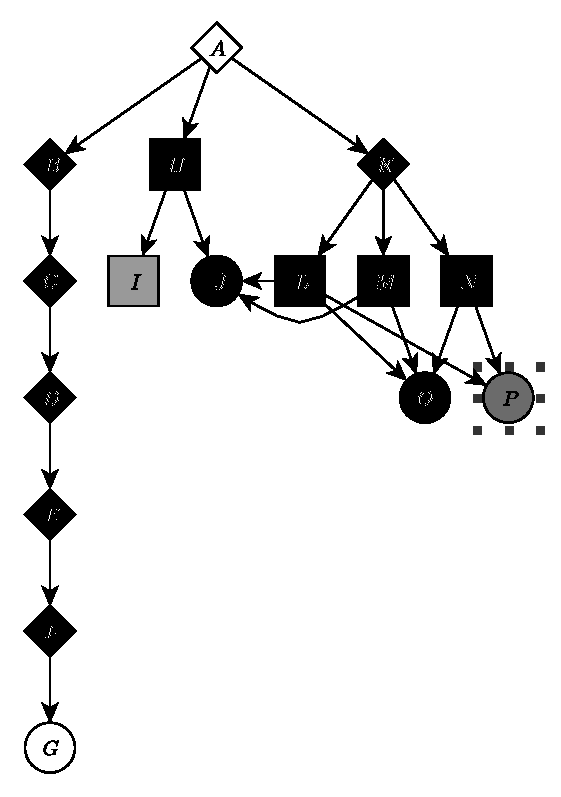
\includegraphics[scale=0.7]{images/trust-beispiel.pdf}
  \caption{Beispiel für die Berechnung der Gültigkeit von Schlüsseln}
  \label{fig:trust-beispiel}
\end{figure}

Abbildung \ref{fig:trust-beispiel} gibt ein Beispiel für die
Berechnung der Gültigkeit von Schlüsseln unter Verwendung der
Standard-Parameter $N=1$, $M=3$ und $L=5$. Die Schlüssel $B, H$ und
$K$ wurden direkt von $A$, dem Besitzer des Schlüsselrings,
unterschrieben und sind deshalb voll gültig. Da $L, M,$ und $N$ von
$K$ unterschrieben wurden und dieser über volles Vertrauen verfügt,
sind sie ebenfalls voll gültig. $O$ sowie $J$ sind voll gültig, da sie
jeweils von drei Schlüsseln mit geringfügigem Vertrauen unterschrieben
wurden. $I$ und $P$ wurden dagegen jeweils nur von zwei Schlüsseln mit
geringfügigem Vertrauen unterschrieben und sind deshalb nicht voll, 
sondern nur eingeschränkt gültig. $G$ wurde zwar von einem voll
gültigen Schlüssel mit vollem Vertrauen unterschrieben. Allerdings
überschreitet die Signaturkette zu $A$ die maximale Länge von 5 und
wird deshalb nicht benutzt.

Ein öffentlicher Schlüssel, der anhand dieser Regeln nicht als
authentisch verifiziert werden kann, kann trotzdem zur Verschlüsselung
und zur Verifizierung von Signaturen verwendet werden. Allerdings
warnt GnuPG in diesem Fall vor der Verwendung.

Es muss bemerkt werden, dass keine direkte Verbindung zwischen dem
Vertrauenswert und dem Gültigkeitswert eines Schlüssels
besteht. Ein Schlüssel, dem voll vertraut wird, kann trotzdem
aufgrund von fehlenden Signaturketten ungültig sein. Signaturen
dieses Schlüssels können dann nicht benutzt werden.

\subsection{Das Keyserver-Netzwerk}
\label{sec:das-keys-netzw}

Die Verbreitung von öffentlichen Schlüsseln ist auf beliebigen Wegen
möglich, etwa per E-Mail oder auf Webseiten. Ein zentraler Ablageort
für öffentliche Schlüssel erleichtert das Auffinden derselben aber
erheblich. Im Kontext von PGP wird diese Aufgabe von \emph{Keyservern}
übernommen. Dabei handelt es sich im wesentlichen um Datenbanken von
OpenPGP-Schlüsseln, die nach verschiedenen Kriterien (etwa nach KeyID
oder UserID) durchsucht werden können. Benutzer können ihre
öffentlichen Schl\"ussel auf diese Keyserver laden, um sie der
Öffentlichkeit zur Verfügung zu stellen.

Schlüssel können von beliebigen Personen auf Keyserver geladen
werden, nicht nur durch die Benutzer. Auf diesem Weg werden auch
Signaturen (also Zertifikate), die durch einen Zertifizierer auf einem
Schlüssel angebracht wurden, verbreitet. Der Zertifizierer lädt
den veränderten Schlüssel auf einen Keyserver. Dieser fügt die
neuen Signaturpakete dem bisherigen Schlüssel hinzu. Dabei werden
stets nur Pakete zu Schlüsseln hinzugefügt, nicht überschrieben
oder gelöscht. Auf diese Weise machen Keyserver den
Zertifikatsgraphen zugänglich. Selbstverständlich können
Zertifikate auch auf anderen (eventuell privaten) Wegen ausgetauscht
werden.

Um Lastverteilung und Fehlertoleranz zu erreichen, existieren mehrere
Keyserver. Diese sind als Netzwerk organisiert und synchronisieren
ihren Datenbestand ständig untereinander. Benutzer finden also auf
allen Keyservern des Netzwerks mit sehr geringer Verzögerung den
gleichen Datenbestand\footnote{In Tests des Autoren dauerte es
  normalerweise weniger als 10 Sekunden, bis neue Schlüssel auf alle
  Keyserver des Verbundes propagiert waren.}. Das öffentliche
Keyserver-Netzwerk besteht derzeit (Mai 2010) aus 48
Keyservern \cite{SKS}. Die üblicherweise
verwendete Keyserver-Software wird in Abschnitt
\ref{ch:Grundlagen:sec:Design:subsec:der-sks-keyserver} beschrieben.

Eine wichtige Eigenschaft des Keyserver-Netzwerks ist es, dass sich
Schlüssel, die einmal auf einen der dazugehörigen Keyserver
abgelegt wurden, nicht mehr aus dem Netzwerk entfernen lassen. Zwar
kann ein Schlüssel oder ein einzelnes OpenPGP-Paket aus der
Datenbank von einzelnen Keyservern gelöscht werden. Allerdings wird
er in diesem Fall durch die Synchronisierung mit anderen Keyservern
des Netzwerks wieder auftauchen. Das Keyserver-Netzwerk insgesamt
sieht keine Prozedur für die Entfernung von Schlüsseln vor. Das
bedeutet, dass das öffentliche Keyserver-Netzwerk alle\footnote{Es
  kann nicht ausgeschlossen werden, dass einzelne Schlüssel durch
  Softwarefehler verloren gingen. Die zahlreichen Kopien des
  Datenbestandes auf den einzelnen Keyservern und die ständige
  Synchronisation machen dies jedoch unwahrscheinlich.} jemals dort
veröffentlichten Schlüssel enthält. Dieses Verhalten stellt
für Benutzer kein wirkliches Problem dar. Der korrekte Weg, um einen
Schlüssel, der aus beliebigen Gründen nicht mehr benutzbar ist,
unbrauchbar zu machen, ist der Widerruf des Schlüssels. Umgekehrt
würde eine Möglichkeit zur Löschung von Schlüsseln einem
Angreifer die Möglichkeit eröffnen, einzelne Schlüsselteile --
beispielsweise Signaturpakete mit Widerrufssignaturen -- zu entfernen
und dadurch eigentlich widerrufene kompromittierte Schlüssel wieder
gültig erscheinen zu lassen.

Der Widerruf eines Schlüssels oder einzelner Schlüsselbestandteile
durch seinen Besitzer kann nur effektiv erfolgen, wenn die Information
über den Widerruf an alle Personen verteilt wird, die den
entsprechenden öffentlichen Schlüssel potentiell
benutzen. Keyserver bieten die Möglichkeit, die Information über
den Widerruf von Schlüsseln zentral und öffentlich verfügbar zu
machen, indem das Widerrufszertifikat auf den Keyservern verfügbar
gemacht wird. Allerdings kann dieses Vorgehen natürlich nur
funktionieren, wenn Benutzer ihren Schlüsselring regelmäßig mit
den Informationen eines Keyservers aktualisieren. Im Fall der
Kompromittierung eines Schlüssels ist die Information aber
zeitkritisch. Anwender sollten dann direkt informiert werden.

Indem ein Benutzer Signaturen auf einem Keyserver zur Verfügung
stellt, macht er Informationen über seine Beziehungen für die
Öffentlichkeit sichtbar. In Abschnitt \ref{sec:soziale-netzwerke}
wird argumentiert, dass die Signaturbeziehungen einer Person ein
Abbild sozialer Beziehungen von unterschiedlicher Art sind. Die rein
topologische Information eines sozialen Netzwerks erlaubt detaillierte
Aussagen über die Rolle einzelner Personen im
Netzwerk \cite{Carrington2005}. Benutzer müssen sich daher bewusst
sein, dass die Benutzung öffentlicher Keyserver einen Verlust von
Privatsphäre mit sich bringt und müssen dies gegenüber einem
möglichen Gewinn an Sicherheit und Bequemlichkeit abwägen.

\subsection{Zustandekommen von Signaturen im Web of Trust}
\label{sec:sozi-komp-des}
Dieser Abschnitt beschreibt, wie Signaturen im Web of Trust
\"ublicherweise zustande kommen.

\subsubsection{Übliche Zertifizierungsprozeduren}
\label{sec:ubliche-zert}

Bis jetzt wurde nur erklärt, dass eine Signatur die
Zusicherung über die Bindung eines Schlüssels an eine Person,
d.h. eine Identität, darstellt. In diesem Abschnitt wird näher
darauf eingegangen, wie solche Zusicherungen \emph{üblicherweise}
zustande kommen.

Bemerkt werden muss, dass der Zertifizierungsprozess im Kontext des
Web of Trust nicht formal definiert ist. Weder der OpenPGP-RFC noch
andere Standarddokumente machen dazu Vorschriften. Nur Certificate
Authorities, die PGP verwenden, und einige wenige Privatpersonen
dokumentieren ihre Verfahren zur Zertifizierung in Form von
so genannten ``Keysigning-Policies''. Außerdem ist dem Autor dieser
Arbeit keine Studie über tatsächlich verwendete Mechanismen
bekannt. Deshalb wird an dieser Stelle nur anekdotische Evidenz
als Eindruck von üblichen Praktiken präsentiert.

Die Person, die eine Signatur erstellt, wird im folgenden mit
\emph{Unterzeichner}, und die Person, deren Schlüssel
unterschrieben wird, mit \emph{Unterzeichneter} bezeichnet. Um
die oben erwähnte Zusicherung abgeben zu können, muss der
Unterzeichner die Identität des Unterzeichneten überprüfen und
so sicherstellen, dass sie mit der auf dem Schlüssel angegebenen
Identität (in Form der \emph{UserID}) übereinstimmt. Diese
Überprüfung sollte in Form eines \emph{persönlichen} Treffens
stattfinden, da sonst eine sinnvolle Identitätsüberprüfung im
Allgemeinen nicht möglich ist. Der Unterzeichnete sollte zuerst den
Fingerabdruck seines Schlüssels präsentieren. Anhand dieses
Fingerabdrucks kann der Unterzeichner überprüfen, dass der zu
unterschreibende Schlüssel tatsächlich der des Unterzeichneten
ist.  Der Unterzeichnete sollte dann ein Dokument präsentieren, dass
seine Identität belegt. Um die Verwendung von gefälschten
Dokumenten zu erschweren, wird üblicherweise ein amtliches
Ausweisdokument mit Lichtbild gefordert (Personalausweis,
Reisepass). Der Unterzeichner kann nun anhand des Dokumentes
überprüfen, dass der Unterzeichner mit der auf dem Schlüssel
vermerkten Identität identisch ist. Damit kann der Unterzeichner den
Schlüssel unterschreiben und die obige Zusicherung
abgeben. Normalerweise werden beide Teilnehmer ihre Schlüssel
gegenseitig unterschreiben, also die Rollen von Unterzeichner und
Unterzeichnetem wechseln.

Dies sind die üblichen Anforderungen an einen
Zertifizierungsprozess, wie sie von ernsthaften Benutzern des Web of
Trust erwartet werden. Allerdings hindert einen Teilnehmer nichts
daran, diese Anforderungen beliebig abzuschwächen. Er kann
beispielsweise auf die Identitätsüberprüfung von Personen
verzichten, die ihm persönlich bekannt sind oder im Extremfall auf
jegliche Überprüfung verzichten. Allerdings ist jeder Benutzer
selbst dafür verantwortlich zu entscheiden, welchen Personen er
dahingehend vertraut, korrekte Zusicherungen abzugeben.

\subsubsection{Certificate Authorities im Web of Trust}
\label{sec:cert-auth-im}

Eine Reihe von Einrichtungen agiert im Kontext des Web of Trust als
\emph{Certificate Authorities} im Sinne von Abschnitt
\ref{ch:Grundlagen:sec:PublicKeyCrypto:subsec:KeyAuth:subsubsec:PKI}. Diese
Einrichtungen bieten als Dienstleistung die Signierung von
PGP-Schlüsseln nach Überprüfung der Identität an. Der Prozess
bzw. die Kriterien, nach dem diese Signaturen zustande kommen, ist
dokumentiert. Dieser Prozess unterscheidet sich üblicherweise nicht
von dem in Abschnitt \ref{sec:ubliche-zert} beschriebenen Vorgehen.

\begin{itemize}
\item Der Heise-Verlag betreibt seit 1997 eine Certificate Authority
  im Rahmen der ``Krypto-Kampagne''. Diese hat sich zum Ziel gesetzt,
  die Verbreitung von PGP zu fördern. Durch eine kostenlose
  Certificate Authority soll das Web of Trust gestärkt werden.

  Die Zertifizierung wird auf Messen gegen Vorlage des
  Personalausweises angeboten. Die von dieser CA verwendeten
  Schlüssel haben insgesamt ca. 22.000 Signaturen erstellt.
\item Die Certificate Authority CACert zertifiziert unter
  anderem auch OpenPGP-Schlüssel. Der von dieser CA verwendete
  Schlüssel hat ca. 3.400 Schlüssel signiert.
\item Das Deutsche Forschungsnetzwerk (DFN) betrieb vermutlich bis zum
  Jahr 2009 eine Certificate Authority für PGP.
\end{itemize}

Das Konzept einer Certificate Authority steht nicht grundsätzlich im
Widerspruch zu dem des Web of Trust. Eine Verifizierungsprozedur wie
in Abschnitt \ref{sec:ubliche-zert} macht für einen Schlüssel
einer Certificate Authority keinen Sinn, da er üblicherweise nicht
mit einer einzelnen Person verbunden ist. Ein Benutzer muss
sicherstellen, dass der CA-Schlüssel authentisch ist und
entscheiden, ob er dem Betreiber dahingehend vertraut, die
dokumentierte Policy zuverlässig umzusetzen. Zusätzlich muss
allerdings der CA-Schlüssel signiert werden, um seine Signaturen
benutzen zu können. Werden diese Signaturen auf dem CA-Schlüssel
veröffentlicht, dann ergeben sich Signaturpfade, die zu diesem
Schlüssel führen. Der CA-Schlüssel kann dann auch von
Teilnehmern, die ihn nicht direkt unterschrieben haben, als Teil ganz
normaler Signaturketten verwendet werden (sofern sie dem Betreiber der
Certificate Authority vertrauen). Certificate Authorities fügen sich
also problemlos in das dezentrale Web of Trust ein.

\subsubsection{Keysigning-Parties}
\label{sec:keysigning-parties}

Das in Abschnitt \ref{sec:ubliche-zert} beschriebene übliche Verfahren
betrifft zunächst nur zwei Personen. Wenn mehrere Personen
zusammenkommen, um ihre Schlüssel gegenseitig zu unterschreiben, wird
von einer \emph{Keysigning-Party} (KSP) gesprochen. Die Bandbreite dieser
Veranstaltungen ist sehr groß. Sie reicht von informellen
Zusammenkünften mehrerer Personen, die paarweise ihre Schlüssel
unterschreiben, bis hin zu größeren, formalisierten Veranstaltungen im
Kontext von Konferenzen und Messen. Für grössere
Veranstaltungen hat sich eine Reihe von ``Protokollen'' etabliert, um
den Ablauf effizient zu organisieren\cite{Brennen2008}.

Grössere Keysigning-Parties Open-Source-Umfeld fanden im Jahr 2009
beispielsweise auf diesen Veranstaltungen statt:
\begin{itemize}
\item Debconf (Konferenz des Debian-Projekts) mit 113 Teilnehmern
\item FOSDEM (Open-Source-Konferenz) mit 253 Teilnehmern
\item LinuxTag (Messe) mit 132 Teilnehmern
\end{itemize}

Offensichtlich ist die Obergrenze der Signaturen, die aus einer
Keysigning-Party mit $n$ Teilnehmern entstehen können, $n^2$. Schon
bei Veranstaltungen mit wenigen hundert Teilnehmern werden also
erhebliche Mengen von Signaturen dem Web of Trust hinzugefügt.

Insbesondere auf kleinen und spontanen Veranstaltungen ist es jedem
Teilnehmer überlassen, mit welchen anderen Teilnehmern er Signaturen
austauscht. Üblich ist allerdings, dass (fast) alle Paare von
Teilnehmern Signaturen austauschen. Ein hervorstechendes Merkmal
vieler Keysigning-Parties ist also eine (fast) vollständige
Vernetzung ihrer Teilnehmer.

\subsubsection{PGP im Debian-Projekt}
\label{sec:foobar-fixme}

In einer Reihe von Open-Source-Projekten spielen PGP und das Web of
Trust eine wichtige Rolle. Im Debian-Projekt beispielsweise werden
PGP-Schlüssel unter anderem benutzt, um alle bereitgestellten
Softwarepakete durch den zuständigen Entwickler signieren zu
lassen. Auf diese Weise wird überprüft, dass ein hochgeladenes
Paket tatsächlich von dem verantwortlichen Projektmitglied stammt
und nicht verändert wurde. Dazu muss jeder der etwa 1000
Debian-Entwickler über einen Schlüssel verfügen, der von
mindestens einem anderen Debian-Entwickler verifiziert und
unterschrieben wurde. Auf diese Weise bildet sich bereits innerhalb
des Projekts ein Web of Trust, das einen Teil des globalen Web of
Trust darstellt. PGP scheint eine wichtige Rolle in der Kultur des
Projekts zu spielen. Darauf weist beispielsweise hin, dass auf Treffen
von Projektmitgliedern oft Keysigning-Parties abgehalten werden, um
das Web of Trust zu stärken. Außerdem signiert eine
überdurchschnittliche Anzahl von Debian-Entwicklern ihre E-Mails auf
projektinternen Mailinglisten.

\section{Graphentheorie und Netzwerkanalyse}
\label{sec:graph-und-netzw}

Dieser Abschnitt erkl\"art f\"ur die weitere Arbeit ben\"otigte
Grundlagen aus Graphentheorie und Netzwerkanalyse.

\subsection{Graphentheorie allgemein}
\label{ch:Grundlagen:sec:Graphentheorie}

Dieser Abschnitt führt einige grundlegende graphentheoretische
Begriffe ein. Er richtet sich nach den Beschreibungen in \cite{Brandes2004}.
  
Ein \emph{Netzwerk} bezeichnet eine Ansammlung von Objekten, zwischen
denen bilaterale Beziehungen bestehen. Das hier betrachtete Netzwerk
besteht aus einer Ansammlung von OpenPGP-Schlüsseln, zwischen denen
Beziehungen in Form von Signaturen bestehen. Ein Netzwerk kann durch einen
Graphen repräsentiert werden.

Ein \emph{Graph} $G=(V, E)$ besteht aus einer endlichen Menge $V$ von
\emph{Knoten} und einer endlichen Menge $E$ von \emph{Kanten}, die je
zwei Knoten miteinander verbinden. Die Anzahl $|V|$ der Knoten wird mit
$n$ und die Anzahl der Kanten mit $m$ bezeichnet. Zwei durch eine
Kante verbundene, \emph{benachbarte} Knoten heißen
\emph{adjazent}. In einem \emph{ungerichteten} Graphen ist $E$ eine
Teilmenge von $V\times V$, also eine Menge von Kanten $\{u, v\}$, die
zwei Knoten $u \in V$ und $v\in V$ verbinden. In einem
\emph{gerichteten} Graphen besteht eine Kante aus einem geordneten
Paar $(u, v)$ von Knoten. Eine gerichtete Kante $(u, v)$ führt vom
\emph{Ursprung} $u$ zum \emph{Ziel} $v$.

Auf Kanten kann eine Funktion $w: E \rightarrow \mathbb{N}$ definiert
sein, die jeder Kante ein \emph{Gewicht} zuordnet. Ein solcher Graph
heißt dann \emph{gewichtet}.

Ein Graph ist \emph{vollständig}, wenn er alle möglichen Kanten
enthält.

Der \emph{Grad} $d(v)$ eines Knotens $v$ in einem ungerichteten
Graphen bezeichnet die Anzahl der Kanten, die diesen Knoten
enthalten. Die \emph{Nachbarschaft} $N(v)$ bezeichnet die Menge der
Knoten, die zu $v$ adjazent sind. In einem gerichteten Graphen
bezeichnet der \emph{eingehende Grad} $d^{-}(v)$ die Anzahl der
Kanten, die den Knoten $v$ als Ziel enthalten, und der
\emph{ausgehende Grad} $d^{+}(v)$ die Anzahl der Kanten, die $v$ als
Ursprung enthalten.

Ein \emph{Kantenzug} zwischen Knoten $v_0$ und $v_k$ in einem Graphen
$G=(V, E)$ ist eine alternierende Folge $(v_0, e_1, v_1, e_2, \dots,
v_{k-1}, e_k, v_k)$, wobei $v_i \in V$, $e_i \in E$, sowie $e_i =
\{v_{i-1}, v_{i}\}$ in einem ungerichteten Graphen bzw. $e_i =
(v_{i-1}, v_{i})$ in einem gerichteten Graphen. Der Kantenzug hat die
\emph{Länge} $i$. Ein Kantenzug heißt \emph{einfach}, wenn $e_i \ne
e_j$ für $i \ne j$ gilt.  Ein einfacher Kantenzug heißt
\emph{Pfad}, wenn $v_0, \dots, v_k$ paarweise verschieden sind. Die
\emph{Distanz} $d(u, v)$ von einem Knoten $u$ zu einem Knoten $v$ ist die
Länge eines kürzesten Pfades zwischen $u$ und $v$. Besteht kein
Pfad von $u$ nach $v$, so wird $d(u,v) = \infty$ definiert.

Ein Graph $G' = (V', E')$ ist ein \emph{Teilgraph} eines Graphen $G =
(V, E)$, wenn $E' \subseteq E$ und $V' \subseteq V$ gelten. Ein
Teilgraph $G' = (V', E')$ eines Graphen $G$ ist durch eine
Knotenmenge $V'$ \emph{induziert}, wenn $E' = \{(u, v) : u \in V, v
\in V, (u, v) \in E\}$ gilt.

Eine \emph{Partitionierung} oder \emph{Zerlegung} eines Graphen
bezeichnet Mengen (auch: \emph{Cluster}) $V_1, \dots, V_n$ mit $V_i
\cap V_j = \emptyset \quad \forall 1 \le i, j \le n$ und $V_1 \cup
\dots \cup V_n = V$. Kanten $(u, v), u \in C_k, v \in C_k$, die
innerhalb einer solchen Menge verlaufen, heißen
\emph{Intraclusterkanten}. Kanten $(u, v), u \in C_k, v \in C_l, k \ne
l$, die zwischen solchen Mengen verlaufen, heißen
\emph{Interclusterkanten}.

Ein ungerichteter Graph heißt \emph{zusammenhängend}, wenn es
zwischen allen Knotenpaaren $u, v$ einen Pfad gibt. Eine
\emph{Zusammenhangskomponente} eines Graphen $G$ ist ein
\emph{maximaler}, zusammenhängender induzierter Teilgraph von
$G$. Ein gerichteter Graph ist \emph{stark zusammenhängend}, wenn es
für jeden Knoten einen gerichteten Pfad zu jedem anderen Knoten gibt. Eine
\emph{starke Zusammenhangskomponente} eines Graphen $G$ ist dann ein
maximaler, stark zusammenhängender induzierter Teilgraph von $G$.

\subsection{Netzwerkstatistiken}
\label{ch:Grundlagen:sec:Netzwerkanalyse:subsec:Statistiken}

In diesem Abschnitt werden einige Kennzahlen nach
\cite{Brinkmeier2004} definiert, die die Struktur eines Graphen
charakterisieren.

Die Distanz zwischen zwei Knoten wurde bereits im vorherigen Abschnitt
definiert. Ausgehend davon können die Distanzen \emph{eines Knotens}
durch die durchschnittliche Distanz dieses Knotens zu allen anderen
Knoten charakterisiert werden:

\begin{equation}
  \label{eq:1}
  \bar{d}(u) = \frac{1}{n-1} \sum_{v \ne u} d(u, v)
\end{equation}

Für einen gesamten Graphen gibt die \emph{charakteristische oder
  durchschnittliche Distanz} den Durchschnitt aller Distanzen in
diesem Graphen an:

\begin{equation}
  \label{eq:2}
  \bar{d} = \frac{1}{n^2 - n} \sum_{u \ne v \in V} d(u, v)
\end{equation}

Die \emph{Eccentricity} eines Knotens $u$ ist definiert als die
maximale Distanz zu einem anderen Knoten, also

\begin{equation}
  \label{eq:3}
  \epsilon(u) = \max\{d(u,v) | v \in V\}
\end{equation}

Davon ausgehend  wird der \emph{Durchmesser} eines Graphen als Maximum
und der Radius als Minimum über die Eccentricity aller Knoten
definiert. Durchmesser und Radius geben also die Ober-
bzw. Untergrenze der Pfadlänge an, mit der ein Knoten alle anderen
Knoten erreichen kann. Bemerkt werden muss, dass alle auf Distanzen
basierenden Kennzahlen im Falle eines nicht (stark)
zusammenhängenden Graphen unendlich sind. Dieses Problem wird im
weiteren vermieden, indem diese Kennzahlen nur für (starke)
Zusammenhangskomponenten berechnet werden.

Als Verallgemeinerung der Nachbarschaft eines Knotens wird die
\emph{h-Nachbarschaft} eines Knotens als
\begin{equation}
  \label{eq:4}
  N_h(v) = \{ u \in V | d(v, u) \le h \}
\end{equation}
definiert, d.h. die Menge der Knoten, zu denen die Distanz von $v$ aus
höchstens $h$ beträgt.

Der \emph{Clustering-Koeffizient} nach Watts und Strogatz ist ein
Ma{\ss}
dafür, wie \emph{transitiv} die Beziehungen in einem Netzwerk
sind. Ein hoher Clustering-Koeffizient steht für eine hohe
Wahrscheinlichkeit, dass zwei Nachbarn $v$ und $w$ eines Knotens $u$
auch untereinander verbunden sind. Sei $G = (V, E)$ ein ungerichteter
Graph. Ein Dreieck $\bigtriangleup = \{V_{\bigtriangleup},
E_{\bigtriangleup}\}$ ist ein vollständiger Teilgraph der Größe 3
von $G$. Die Anzahl der Dreiecke \emph{eines Knotens} wird mit
$\lambda(v) = |\{\bigtriangleup : v \in V_{\bigtriangleup}\}|$
bezeichnet. Ein \emph{Tripel} an einem Knoten $v$ ist ein Teilgraph
von $G$ bestehend aus 2 Kanten sowie $v$ und 2 weiteren Knoten, so
dass beide Kanten $v$ enthalten. Die Anzahl der Tripel eines Knotens
$v$ kann durch den Grad $d(v)$ ausgedrückt werden als
$\tau(v)=\binom{d(v)}{2}$. Der \emph{lokale} Clustering-Koeffizient
$c_v$ eines Knotens wird dann als
\begin{equation}
  \label{eq:5}
  c(v) = \frac{\lambda(v)}{\tau(v)}
\end{equation}
definiert. $c(v)$ gibt also an, wie viele der
möglichen Dreiecke an $v$ auch tatsächlich Dreiecke sind. Der
globale Clustering-Koeffizient von $G$ ist dann
\begin{equation}
  \label{eq:6}
  C(G) = \frac{1}{|V'|} \sum_{v \in V'}c(v)
\end{equation}
wobei $V' = \{v \in V : d(v) \ge 2\}$ gesetzt wird, um nicht
definierte Werte für $\tau(v)$ zu vermeiden.

Pastor-Satorras et al. definieren ein Ma{\ss} für die Korrelation der
Knotengrade in einem Netzwerk \cite{PhysRevLett.87.258701}. Der Wert
\begin{equation}
  \label{eq:9}
  <knn> = \sum_{k'} k'P_c (k'|k)
\end{equation}
gibt den durchschnittlichen Grad der Nachbarn von Knoten mit Grad $k$
an.  Dabei gibt die bedingte Wahrscheinlichkeit $P_c(k'|k)$ die
Wahrscheinlichkeit an, dass eine Kante, die an einem Knoten mit Grad
$k$ beginnt, an einem Knoten mit $k'$ endet.

Ein verwandtes Ma{\ss} wird von Newman eingeführt: Ein Netzwerk zeigt
\emph{assortative mixing}, wenn Knoten mit hohem Grad hauptsächlich
mit solchen Knoten verbunden sind, die ebenfalls einen hohen Grad
haben\cite{PhysRevLett.89.208701}. Diese Eigenschaft wird durch den
\emph{Assortativity-Koeffizienten} (ebd.)  gemessen, dessen Werte
zwischen -1 und 1 liegen. Positive Werte für ein Netzwerk zeigen
assortative mixing an, bei negativen Werten zeigt das Netzwerk kein
assortative mixing. Newman gibt an, dass assortative mixing eine
Eigenschaft ist, die viele soziale Netzwerke von anderen Netzwerken --
etwa technischer oder biologischer Natur unterscheidet. Die
meisten sozialen Netzwerke zeigen assortative mixing, während die
restlichen dies nicht tun.

\subsection{Soziale Netzwerke}
\label{sec:soziale-netzwerke}

Ein \emph{soziales Netzwerk} ist nach \cite{newman:167} eine
Menge von Personen bzw. Gruppen von Personen, zwischen denen
Beziehungen bzw. Kontakte bestehen. Die Art dieser Interaktionen ist
dabei beliebig: Beispiele f\"ur soziale Netzwerke, die in der Literatur analysiert
wurden, sind unter anderem Freundschaftsnetzwerke von Schulkindern, Netzwerke
von sexuellen Kontakten und Netzwerke von Geschäftsbeziehungen
(ebd.).

Die im Web of Trust vorhandenen Schlüssel können als
Repräsentationen der Besitzer dieser Schlüssel aufgefasst
werden. Allerdings ist dies keine Eins-zu-eins-Beziehung, da eine
Person über beliebig viele Schlüssel verfügen kann. Die
Beziehung dieser Personen im Web of Trust repräsentiert zunächst
nur eine Signatur, also eine Zusicherung über die Bindung zwischen
dem signierten Schlüssel und der Identität des Besitzers. Es
scheint allerdings recht unwahrscheinlich, dass solche Signaturen
zwischen Personen entstehen, die sich völlig unbekannt sind und in
keiner Beziehung zueinander stehen. Stattdessen wird in dieser Arbeit
davon ausgegangen, dass sich Signaturen in den meisten Fällen anhand
von bereits bestehenden sozialen Kontakten zwischen den Besitzern der
Schlüssel ergeben \cite{Capkun2002}. Das Spektrum möglicher
Beziehungen ist dabei natürlich sehr weit und umfasst mindestens
alle Gruppen von Personen, die potentiell ein Interesse an
vertraulicher und authentifizierter E-Mail-Kommunikation haben: Es
kann sich dabei um persönliche Bekanntschaften handeln, also etwa um
Freunde und Bekannte. Genauso kann sich die Beziehung auch primär
durch die Mitgliedschaft in einer gemeinsamen Gruppe oder Institution
ergeben. Denkbar sind hier zum Beispiel Beziehungen, die sich aus
Arbeitsverhältnissen oder einer Ausbildung ergeben, also Unternehmen
oder akademische Einrichtungen. Genauso gut kann es sich aber um die
Mitgliedschaft in einem Open-Source-Projekt, einem Verein oder einer
politischen Organisation handeln. Auch Zusammenhänge, die nicht
über eine formale Mitgliedschaft in einer festen Gruppierung
entstehen, sind möglich.

Zumindest im Fall von größeren, formalen Keysigning-Parties scheint
zunächst nicht notwendigerweise eine Verbindung zwischen den
Teilnehmern (abgesehen von der Teilnahme selbst) zu bestehen. Es ist
aber auch der Kontext relevant, in dem die Keysigning-Party
stattfindet. Bei einer Konferenz oder Messe kann es sich um ein
Ereignis mit einer klar definierten Zielgruppe handeln, die wiederum
einer Gruppe zuordenbar ist (z.B. im Fall der
``Debconf''-Konferenzen). Ist dies nicht möglich, so handelt es sich
immerhin um eine Gruppe von Personen, die über ein gemeinsames
Interessengebiet verfügen (beispielsweise im Fall der
``LinuxTag''-Keysigning-Parties).

\subsection{Small-World-Effekt}
\label{sec:small-world-effekt}

In sozialen Netzwerken tritt fast immer das Ph\"anomen auf, dass die
die Distanzen zwischen den meisten Knotenpaaren in Relation zur
Gr\"o{\ss}e des Netzwerks sehr gering sind \cite{newman:167}. Dieser Effekt wird als
Small-World-Effekt bezeichnet. Der Begriff geht auf ein Experiment von 
Milgram zur\"uck, bei dem Briefe von Person zu
Person\footnote{Teilnehmer wurden aufgefordert, die Briefe an ihnen
  direkt bekannte Personen weiterzugeben, von denen sie annahmen, dass
  sie sich ``näher'' am Ziel befinden würden.} weitergegeben
wurden, um sie von zufällig ausgewählten Absendern zu ebenfalls
zufällig ausgewählten, geographisch weit entfernten Empfängern
zu transportieren\cite{Travers1969}. Diese Briefe erreichten ihr Ziel
im Durchschnitt über nur sechs Zwischenstationen\footnote{71\% der
  Briefe erreichten ihr Ziel nicht.}. Mit diesem Experiment wurde
gezeigt, dass Paare von Akteuren in einem sozialen Netzwerk nur durch
wenige ``Zwischenschritte'' miteinander verbunden
sind. Eine präzisere Formulierung
ist, dass die durchschnittliche Distanz nur logarithmisch mit der
Anzahl der Knoten wächst.

Auch zufällige Graphen nach dem $G_{n,p}$-Modell verfügen über eine geringe
durchschnittliche Distanz \cite{Baumann2004}. Strogatz und Watts bemerken, dass viele
reale Netzwerke zusätzlich über ausgeprägtes Clustering
verfügen, also über einen hohen
Clustering-Koeffizienten \cite{Watts1998}.

\subsection{Skalenfreie Netzwerke}
\label{sec:skal-netzw}

Eine Verteilung $p$ folgt einem \emph{power law}, wenn sie die Form

\begin{equation}
  \label{eq:8}
  p(k) = ck^{-\delta} \quad \delta > 0, c > 0
\end{equation}
hat \cite{Baumann2004}. Damit kommen kleine Werte häufig vor,
während sehr große Werte nur sehr selten vorkommen.  Ein zentrales
Merkmal solcher Verteilungen ist eine hohe
\emph{Variabilität}. Damit ist gemeint, dass die Abweichungen vom
Durchschnittswert sich um mehrere Größenordnungen unterscheiden
können, so dass der Durchschnitt nicht besonders aussagekräftig
ist.

Ein Netzwerk, in dem die Verteilung der Knotengrade zumindest
asymptotisch einem power law
folgt, wird als \emph{skalenfrei} bezeichnet. Dieser Begriff geht auf
Barabasi und Albert zurück, die feststellten, dass eine Reihe von
Netzwerken aus verschiedenen Bereichen -- etwa technologische, soziale
oder biologische Netzwerke -- diese Eigenschaft
aufweisen \cite{Barabasi1999}.

Skalenfreien Netzwerken wird eine Reihe von allgemeinen Eigenschaften
zugeschrieben. Die wichtigste Eigenschaft ist, dass skalenfreie
Netzwerke sehr gut verbundene \emph{Hubs}, also Knoten mit sehr hohem
Grad, enthalten. Diese halten das Netzwerk zusammen und sorgen
dafür, dass das Netzwerk bei der gezielten Entfernung dieser Hubs
sehr schnell zusammenbricht. Auf der anderen Seite sollen sich
skalenfreie Netzwerke sehr robust gegenüber der zufälligen
Entfernung von Knoten zeigen, da die Chance, dabei einen Knoten mit
niedrigem Grad zu treffen, hoch ist \cite{Albert2000}.

\subsection{Communities}
\label{ch:Grundlagen:sec:Netzwerkanalyse:subsec:Communities}

Dieser Abschnitt führt den Begriff der \emph{Community} ein,
definiert das Gütemass \emph{Modularity} und beschreibt einige
Algorithmen zur Erkennung von Communities in Netzwerken. Sofern nicht
anders angegeben, wurde als Quelle ein Übersichtsartikel von
Fortunato \cite{Fortunato2010} benutzt.

\subsubsection{Grundlegende Begriffe}
\label{sec:grundl-begr}

In vielen -- insbesondere sozialen -- Netzwerken neigen die Teilnehmer
dazu, \emph{Gruppen} zu bilden. In sozialen Netzwerken bilden sich
etwa Gruppen von Teilnehmern, die über familiäre,
freundschaftliche oder professionelle Beziehungen miteinander
verbunden sind. Ein besonders intensiv untersuchter Typ solcher
Netzwerke entsteht aus Kooperations- oder Koautornetzwerken von
Wissenschaftlern, in denen sich Wissenschaftler nach ihren
Fachgebieten gruppieren. Andere Beispiele von Netzwerken, in denen
Gruppenbildung stattfindet, sind Netzwerke aus der Biologie,
beispielsweise Netzwerke von Protein-Protein-Interaktionen, in denen
sich funktionell ähnliche Proteine gruppieren, die an den gleichen
biologischen Prozessen teilnehmen. Das hier zentrale Merkmal dieser
Gruppen oder \emph{Communities} ist die Tatsache, dass Mitglieder
einer Gruppe normalerweise deutlich mehr Beziehungen zu anderen
Mitgliedern dieser Gruppe haben als zu Teilnehmern außerhalb. Eine
solche Community sollte sich also auch in der Struktur des Graphen
wiederfinden, der das Netzwerk beschreibt. In der Tat teilen viele --
insbesondere die oben angeführten -- Beispiele von Netzwerken die
Eigenschaft, dass die Kanten des Netzwerks nicht gleichmäßig
verteilt sind. Stattdessen finden sich Gruppen von Knoten, in denen
eine hohe Dichte von Kanten herrscht, während zwischen diesen
Gruppen nur wenige Kanten bestehen.

In der Literatur scheint keine strenge Definition einer Community zu
existieren, die allgemein akzeptiert ist. Stattdessen wird ein
intuitives Verständnis verwendet, nach dem Communities \emph{dichte}
Teilbereiche eines Graphen sind, also Gruppen von Knoten, die
untereinander ``viele'' Kanten haben, während zu nicht in der Gruppe
liegenden Knoten nur ``wenige'' Kanten bestehen. Oft wird werden
Communities auch algorithmisch definiert: Communities sind gerade das
Ergebnis eines Algorithmus zur Community-Zerlegung.

Da ein Graph über ein konkretes Netzwerk abstrahiert und nur noch
die Struktur abbildet, werden auch bei der Community-Erkennung nur
Informationen benutzt, die in der Topologie des Graphen kodiert sind. 

\subsubsection{Algorithmus von Girvan/Newman}
\label{sec:algor-von-girv-1}

An dieser Stelle wird der Algorithmus von Girvan
und Newman\cite{Newman2004} zur Berechnung einer Community-Zerlegung
beschrieben, da er den Startpunkt des großen Interesses in
Community-Algorithmen in den letzten Jahren darstellt.

\emph{Edge betweeness} ist ein auf Kanten definiertes
Zentralitätsma\ss, das auf dem Zentralitätsma\ss \emph{Vertex
  betweeness} \cite{Koschutzki2004a} basiert. Die edge betweeness
einer Kante gibt an, wie hoch der Anteil kürzester Pfade ist, die
diese Kante enthalten, wie wichtig also diese Kante für den
Zusammenhalt und die Distanzen im Netzwerk ist.

Der Algorithmus von Girvan und Newman basiert auf der folgenden Idee:
Wenn Knoten in Communities organisiert sind, dann gibt es nur
vergleichsweise wenige Kanten, die \emph{zwischen} Communities
verlaufen. über diese Kanten müssen alle kürzesten Pfade
zwischen Knoten laufen, die in unterschiedlichen Communities
liegen. Diese Kanten sollten also einen hohen betweeness-Wert
haben. Eine Zerlegung in Communities kann dann berechnet werden, indem
diejenigen Kanten entfernt werden, die Communities verbinden, also
solche mit hoher edge betweeness.

Der Algorithmus führt iterativ die folgenden Schritte aus:

\begin{enumerate}
\item Berechne edge betweeness für alle vorhandenen Kanten.
\item Entferne die Kante mit dem höchsten betweeness-Wert.
\item Kehre zurück zu Schritt 1, solange Kanten vorhanden sind.
\end{enumerate}

Werden genug Kanten entfernt, zerfällt ein Graph in Komponenten, die
\emph{mögliche} Communities darstellen. Da jede Komponente selbst
wieder unterteilt wird, ergibt sich so eine Hierarchie von
Komponenten, die als Baum (ein so genanntes \emph{Dendrogramm})
dargestellt werden können. Ein horizontaler Schnitt durch diesen
Baum auf einer beliebigen Ebene liefert eine Zerlegung des Graphen.

Die Komplexität des Algorithmus beträgt $\mathcal{O}(m^2n)$ für
einen Graphen mit $n$ Knoten und $m$ Kanten. Er ist also für
grössere Graphen nicht geeignet.

\subsubsection{Modularity}
\label{sec:modularity}

Eine solche hierarchische Zerlegung macht noch keine Aussage
darüber, wie ``gut'' die Zerlegung auf einer bestimmten Ebene die
tatsächliche Community-Struktur wiedergibt. Um diese Frage zu
beantworten, wurde ebenfalls von Girvan und Newman als Ma{\ss} für die
Qualität einer Zerlegung die so genannte \emph{Modularity}
definiert \cite{Newman2004}. Gegeben einen ungerichteten Graphen $G=(V,
E)$ und eine Zerlegung dieses Graphen $\mathcal{C} = C_1, ..., C_n$
wird die Modularity $Q$ definiert als
\begin{equation}
  \label{eq:modularity}
  Q =
  \frac{1}{2m}\sum_{u, v \in
    V}\left(A_{uv}-\frac{d(u)d(v)}{2m}\right)\delta\left(C_u, C_v\right)
\end{equation}

Dabei ist $A$ die Adjazenzmatrix von $G$. $C_u$ gibt die Community an,
in der sich der Knoten $u$ befindet. Das Kronecker-Delta $\delta$
ist 1 wenn $C_u = C_v$ gilt, ansonsten 0.

Wenn der Term $\frac{d(u)d(v)}{2m}$ ignoriert wird, läuft die Summe
über alle Kanten, deren Endpunkte sich in der selben Community
befinden. Der gesamte Term gibt dann den Anteil der Kanten an, die
innerhalb einer Community verlaufen (Intraclusterkanten). Ist dieser Anteil groß, so gibt
die Zerlegung die Community-Struktur des Graphen gut
wieder. Allerdings wird das Maximum $Q = 1$ im trivialen Fall $C_1 =
V$ erreicht. Aus diesem Grund wird die Anzahl der Kanten in
Communities zusätzlich mit einem Nullmodell verglichen. Es wird
davon ausgegangen, dass ein zufälliger Graph keine ausgeprägte
Community-Struktur hat. Als Nullmodell wird ein Graph gewählt, bei
dem die Enden der Kanten zufällig gewählt wurden, allerdings so,
dass die Grade der einzelnen Knoten die gleichen wie in $G$ sind.  Die
Wahrscheinlichkeit, dass in einem solchen Graph eine Kante zwischen
Knoten $u$ und $v$ besteht, ist gerade $\frac{d(u)d(v)}{2m}$. $Q$ wird
also dann groß, wenn die \emph{tatsächliche} Anzahl der
Intraclusterkanten höher ist als die \emph{erwartete}.

Brandes et al. haben gezeigt, dass das Problem der Berechnung des
Maximums von $Q$ für einen gegebenen Graphen NP-vollständig
ist \cite{DBLP:journals/tkde/BrandesDGGHNW08}. Eine direkte Berechnung
einer Zerlegung eines Graphen mit maximaler Modularity ist also
vermutlich nicht praktikabel.

Verschiedene Autoren haben Erweiterungen der Modularity-Definition auf
andere Graphen- und Zerlegungstypen vorgeschlagen: etwa für
überlappende Communities \cite{Nicosia2009} und für gerichtete
Graphen \cite{Leicht2008}.

\subsubsection{Weitere Algorithmen}
\label{sec:algorithmen}

Seit der Arbeit von Girvan und Newman wurde eine Vielzahl weiterer
Methoden zur Erkennung von Communities vorgestellt. An dieser Stelle
werden 2 Methoden näher beschrieben, die in dieser Arbeit verwendet
werden. Einen Gesamtüberblick bietet ein Übersichtsartikel von
Fortunato \cite{Fortunato2010}.

\paragraph{Algorithmus von Blondel et al.}
\label{sec:algor-von-blond}

Blondel et al.\cite{Blondel2008} stellen einen Algorithmus vor, der
auf \emph{gierige} Art die Modularity optimiert.  Als
Bewertungsfunktion dient dabei ebenfalls Modularity. Der Algorithmus
funktioniert auf gewichteten Graphen. Dafür wird eine angepasste
Definition der Modularity für gewichtete Graphen
verwendet \cite{Newman2004a}.

Der Algorithmus verläuft in Phasen, die in 2 Schritte aufgeteilt
sind. Im Anfangszustand wird jedem Knoten eine eigene Community
zugewiesen. In jeder Phase wird dann im ersten Schritt in einem
sequentiellen Durchlauf jeder Knoten der Community desjenigen
Nachbarn zugewiesen, für den sich der maximale Zugewinn an
Modularity ergibt. Im zweiten Schritt wird jede der so erhaltenen
Communities zu einem neuen \emph{Superknoten} verschmolzen. Zwischen
zwei Superknoten gibt es genau dann eine Kante, wenn zwischen zwei
ursprünglichen Knoten in den entsprechenden Communities eine Kante
verläuft. Das \emph{Gewicht} dieser \emph{Superkante} ist die Summe
der Gewichte der ursprünglichen Kanten. Die nächste Phase besteht
aus der Anwendung derselben zwei Schritte auf den erhaltenenen
\emph{Supergraphen}. Durch die Phasen ergibt sich wieder eine
Hierarchie in Form eines Baumes. Im Unterschied zum Algorithmus von
Girvan und Newman ist dieser Algorithmus allerdings nicht
\emph{zerteilend}, sondern \emph{verschmelzend}, so dass der Baum von
unten aufgebaut wird.

Der Algorithmus hat eine Komplexität von $O(m)$ und ist damit auch
für sehr große Graphen geeignet.

\paragraph{COPRA}
\label{sec:copra}

Ein gänzlich anderer Ansatz, der nicht direkt mit der Optimierung
des Modularity-Wertes arbeitet, wird von COPRA \cite{Gregory2010}
verwendet. COPRA basiert auf einem Algorithmus von Raghavan et
al. \cite{Raghavan2007}, der auf der Propagierung von \emph{Labels}
beruht. 

Im Anfangszustand wird jedem Knoten ein unterschiedliches Label
zugewiesen. In jeder Iteration wird dann ein sequentieller Lauf in
zufälliger Reihenfolge über alle Knoten durchgeführt. Dabei
übernimmt jeder Knoten das Label, das die Mehrheit seiner Nachbarn
besitzt. Wenn dabei ein Gleichstand auftritt, wird eines der Labels
zufällig ausgewählt. Auf diese Weise werden Labels über den
Graphen propagiert. Einige Labels verschwinden, während andere sich
ausbreiten. Da zwischen Communities nur wenige Kanten bestehen
sollten, ist die Chance, dass sich Labels über Community-Grenzen
ausbreiten, sehr gering. \emph{Innerhalb} von dicht vernetzten Gruppen
sollte sich jedoch ein ``Konsens'' über ein Label ergeben. Das
Konvergenzkriterium besteht darin, dass jeder Knoten ein Label hat,
das von der Mehrheit seiner Nachbarn geteilt wird. Die
Zeitkomplexität des Algorithmus wird durch die Autoren als
``annähernd linear'' angegeben. Er ist also auch für große
Graphen geeignet. Zu beachten ist, dass der Algorithmus durch die
zufällige Reihenfolge, in der die Knoten durchlaufen werden, und die
Auflösung von Pattsituationen \emph{nicht-deterministisch} ist.

Der Algorithmus von Raghavan et al. liefert eine Zerlegung mit
disjunkten Teilmengen von $V$. COPRA verallgemeinert diesen Ansatz zur
Berechnung \emph{überlappender} Communities. Dabei kann ein Knoten
in mehreren Communities enthalten sein, die Teilmengen der Zerlegung
sind nicht mehr disjunkt. Statt einfacher Labels werden Paare $(c, b)$
von Labels $c$ und einem Zugehörigkeitskoeffizienten $b$
propagiert. $b$ drückt aus, wie stark ein Knoten zur Community $c$
gehört. In jedem Schritt übernimmt ein Knoten statt eines einzigen
Labels \emph{alle} Label seiner Nachbarn. Der
Zugehörigkeitskoeffizient eines Knotens $u$ zu Label $c$ in der
Iteration $t$ ist definiert als
\begin{equation}
  \label{eq:10}
  b_t(c, u) = \frac{1}{d(u)}\sum_{v \in N(u)}b_{t-1}(c, v)
\end{equation}
also der Durchschnitt der Zugehörigkeitskoeffizienten aller
Nachbarn für das Label $c$ in der vorherigen Iteration. Die Summe
der Zugehörigkeitskoeffizienten für alle Label eines Knotens
beträgt 1. Um zu vermeiden, dass sich alle Labels ausbreiten, werden
Paare $(c, b)$ gelöscht, wenn $b$ unter einem Schwellwert
$\frac{1}{v}$ liegt. $v$ gibt damit an, in wie vielen Communities ein
Knoten maximal Mitglied sein kann. 

Die Zeitkomplexität von COPRA wird mit $\mathcal{O}(v^3n)$
angegeben, ist also im wesentlichen linear.

%% ==============================
\section{Verwandte Arbeiten}
%% ==============================
\label{ch:Grundlagen:sec:RelatedWork}

An dieser Stelle wird nur auf Arbeiten eingegangen, die sich mit der
Netzwerkstruktur des Web of Trust bei PGP beschäftigen. Für einen
Überblick über Arbeiten zur Struktur von anderen Netzwerken sei auf
\cite{newman:167} und für Arbeiten zur Community-Struktur von anderen
Netzwerken auf \cite{Fortunato2010} verwiesen.

Capkun et al. \cite{Capkun2002} untersuchten strukturelle Aspekte der
größten starken Zusammenhangskomponente eines PGP-Netzwerkes aus dem
Jahr 2001. Dieses Netzwerk zeigte eine geringe charakteristische
Distanz und einen hohen Clustering-Koeffizienten. Außerdem stimmte die
Verteilung der aus- und eingehenden Grade mit einem Power-Law
überein. Die Autoren argumentieren, dass Netzwerke, die aus
Zertifikatsbeziehungen entstehen, naturgemäß den Small-World-Effekt
zeigen, da sich die Zertifikate anhand schon bestehender
Vertrauensbeziehungen ergeben. Die Autoren geben außerdem noch ein
Netzwerkmodell an, das Graphen erzeugen soll, die in den
beschriebenen Charakteristiken dem PGP-Netzwerk ähneln.

Arenas et al. \cite{Boguna2004} analysierten ein PGP-Netzwerk aus dem
gleichen Jahr. Das Netzwerk wurde von vornherein in ein ungerichtetes
Netzwerk umgewandelt, indem nicht gegenseitige Kanten entfernt
wurden. Sie betrachteten die Gradverteilung, den
Clustering-Koeffizienten und die Korrelation von Graden benachbarter
Knoten. Dabei folgt die Verteilung der Knotengrade einem
Power-Law. Der Clustering-Koeffizient des Netzwerkes beträgt $C=0.4$,
ist also recht hoch. Die Grade benachbarter Knoten sind positiv
korreliert. Außerdem benutzten die Autoren den Algorithmus von Girvan
und Newman \cite{Newman2004}, um eine Community-Zerlegung des Netzwerks
zu berechnen. Die Verteilung der Größe dieser Communities folgt wieder
einem Power-Law.

Warren et al. betrachteten das Netzwerk nicht zu einem festen
Zeitpunkt sondern untersuchten die \emph{Dynamik} des
Netzwerks \cite{Warren2007}. Sie berechneten verschiedene grundlegende
Netzwerkeigenschaften (Größe des Netzwerkes, Distanzen,
Gradverteilung etc.) und verfolgten deren Entwicklung \emph{über die
  Zeit}. Ihre Ergebnisse können allerdings mit den in dieser Arbeit
präsentierten nicht verglichen werden, da der Graph von Schlüsseln
auf Individuen reduziert wurde (siehe auch Abschnitt
\ref{sec:schl-und-invid}).

Neben diesen akademischen Arbeiten gibt es mehrere Ansätze aus der
PGP-Community, die Netzwerkstruktur zu untersuchen. Das
wotsap-Projekt \cite{Cederlof} stellt einen täglich aktualisierten
Datensatz bereit, der die Vernetzungsstruktur der größten starken
Zusammenhangskomponente des Web of Trust darstellt. Diese Daten werden
für eine Webapplikation benutzt, die kürzeste Pfade
zwischen Schlüsseln berechnet und visualisiert und so bei der
Nutzung von Zertifikatspfaden behilflich sein soll. In Abschnitt
\ref{ch:Grundlagen:sec:WarumEigene} wird der Wotsap-Datensatz näher
betrachtet und begründet, warum er in dieser Arbeit nicht verwendet
wurde. 

Henk P. Penning berechnet anhand der Wotsap-Daten regelmäßig
strukturelle Eigenschaften des Web of Trust bzw. von dessen größter
starker Zusammenhangskomponente \cite{Penning}. Dies beinhaltet die
Entwicklung der Größe dieser Komponente und der durchschnittlichen
Distanzen über die Zeit, die Verteilung der Knotengrade und die
Verteilung durchschnittlicher Distanzen pro Knoten. Außerdem wird die
Robustheit des Netzwerkes bei der Entfernung von zufällig
ausgewählten bzw. besonders gut vernetzten Knoten simuliert.

%%% Local Variables: 
%%% mode: latex
%%% TeX-master: "diplarb"
%%% End: 
